\documentclass{article}
\usepackage[utf8]{inputenc}

\title{CSE3666 — Lab 5}
\author{Mike Medved}
\date{March 7th, 2022}

\usepackage{color}
\usepackage{caption}
\usepackage{amsthm}
\usepackage{amssymb} 
\usepackage{amsmath}
\usepackage{listings}
\usepackage{listings}
\usepackage{graphicx}
\usepackage[margin=1in]{geometry} 
\usepackage[scaled=0.85]{FiraMono}
\usepackage[table]{xcolor}

\newcommand*\BitAnd{\mathbin{\&}}
\newcommand*\BitOr{\mathbin{|}}
\newcommand*\ShiftLeft{\ll}
\newcommand*\ShiftRight{\gg}
\newcommand*\BitNeg{\ensuremath{\mathord{\sim}}}

\lstset{basicstyle=\ttfamily, keywordstyle=\bfseries}
\lstset{
    language=[LaTeX]TeX,
    aboveskip=3mm,
    belowskip=3mm,
    showstringspaces=false,
    columns=flexible,
    basicstyle={\small\ttfamily},
    numbers=none,
    numberstyle=\tiny\color{gray},
    keywordstyle=\color{blue},
    commentstyle=\color{dkgreen},
    stringstyle=\color{mauve},
    breaklines=true,
    breakatwhitespace=true,
    tabsize=3
}

\definecolor{dkgreen}{rgb}{0,.6,0}

\begin{document}
\graphicspath{ {.} }

\maketitle

\section{Prompt}
In this lab, we implement a 1-bit ALU in MyHDL.

$\hfill \break$
The circuit diagram of 1-bit ALU is shown below. If the link does not work, the file, alu1.svg, is in the same directory as this file.

$\hfill \break$
\begin{center}
    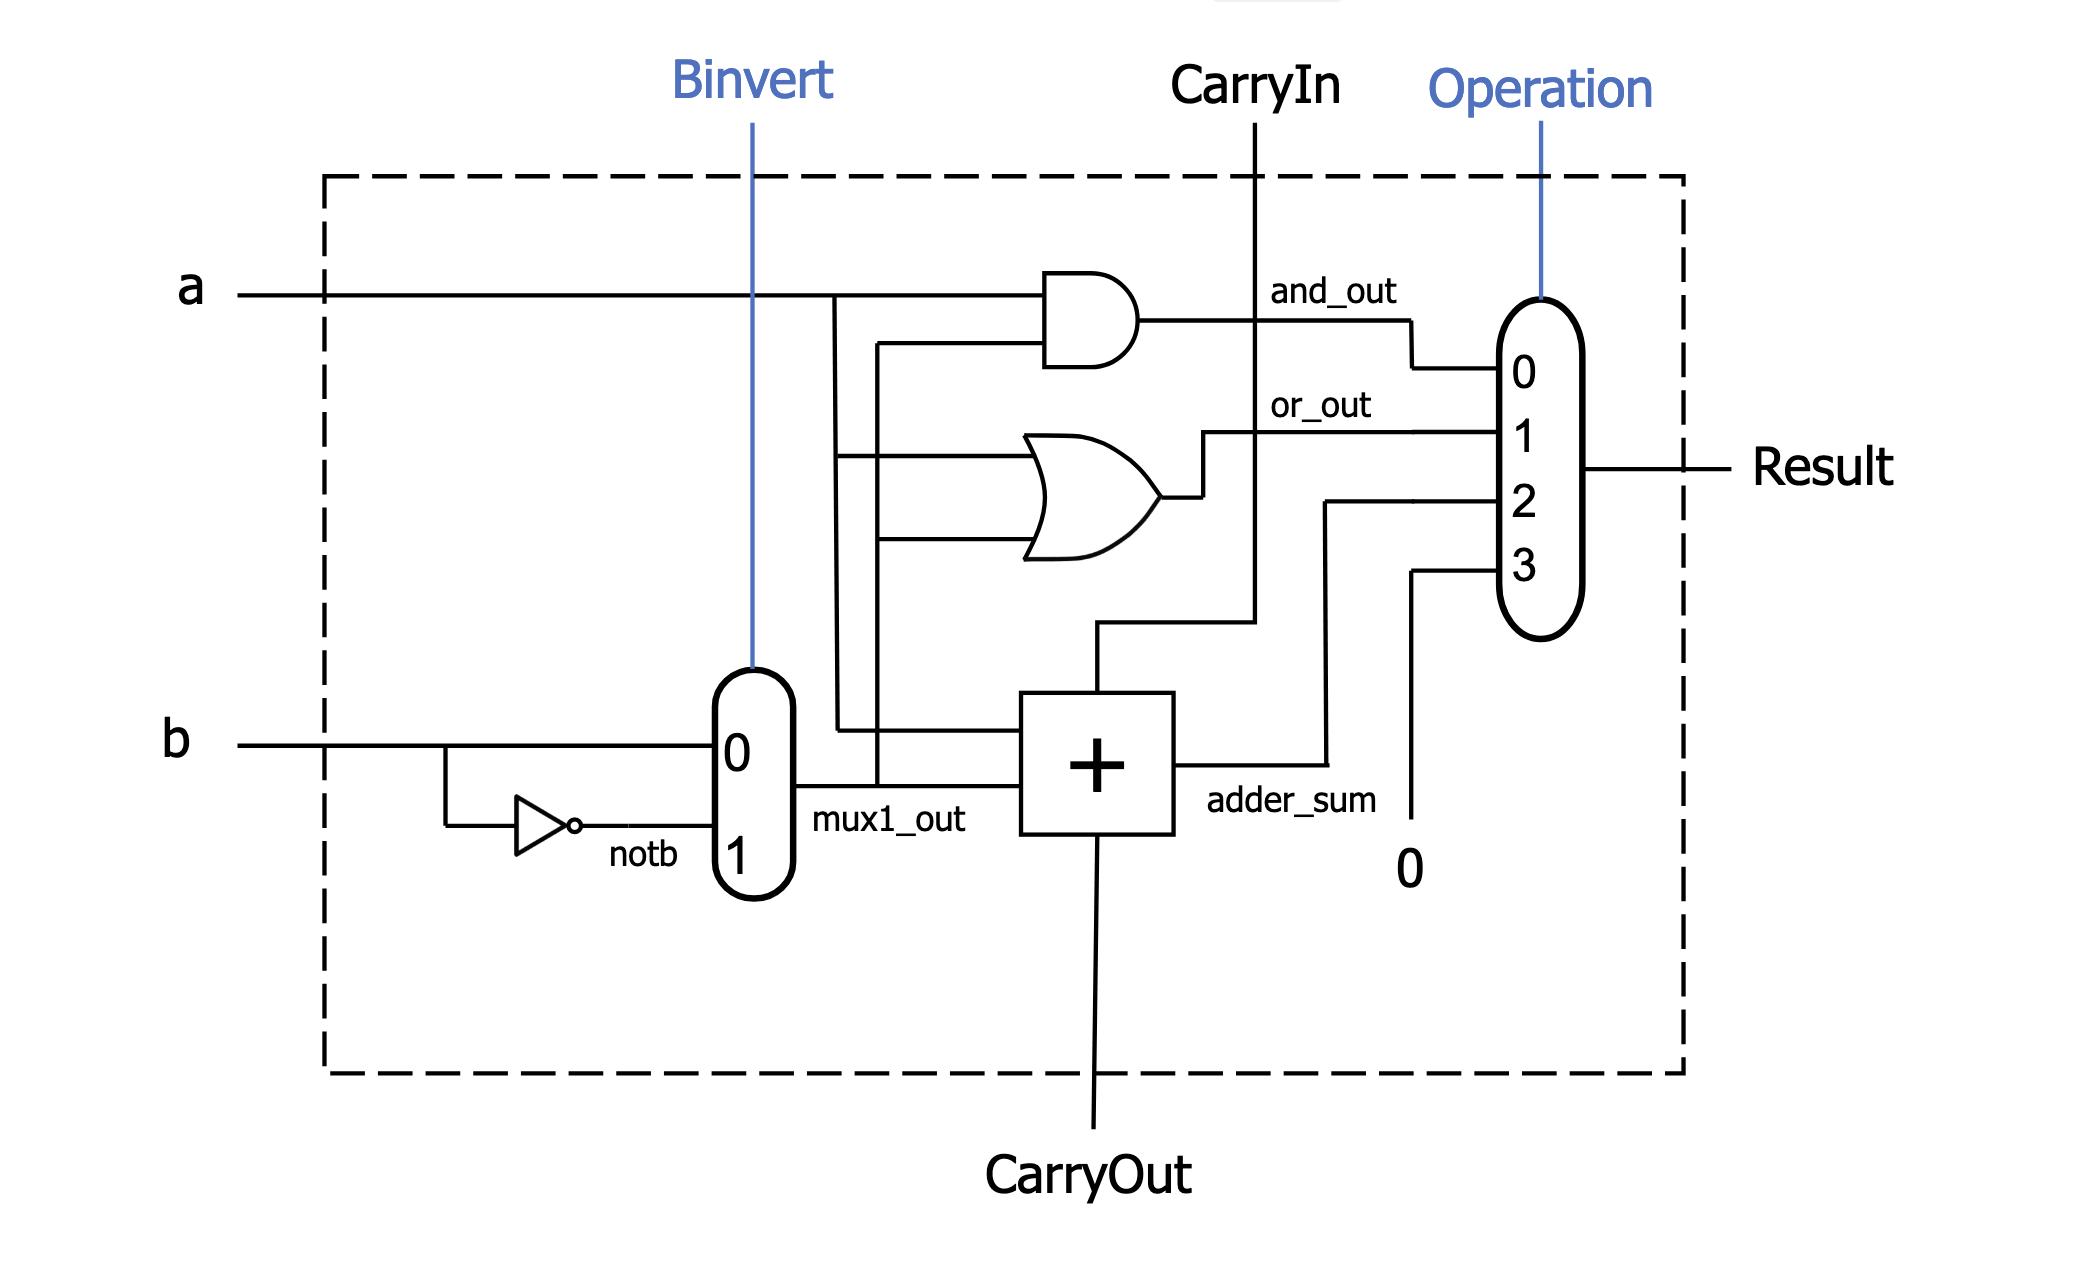
\includegraphics[width=15cm]{alu1.png}
\end{center}

$\hfill \break$
The skeleton code is in alu1.py. Place all logic in alu1\_logic() function. The function in the skeleton code does not change any output signals.

$\hfill \break$
\textbf{Steps}
\begin{enumerate}
    \item \textbf{Study the diagram}
    $\hfill \break$
    All signals are named. Identify internal signals. Internal signals are signals generated in the module (ALU), and used only in the module. For example, notb and mux1\_out are internal signals.
    
    \textbf{List all internal signals in your report.}
    
    Why do we need to identify internal signals? In our code, we do not keep internal signals in MyHDL Signal class because they do not affect other modules/functions.
    
    In later labs, you may have to name signals yourself. Do NOT use the same name for different signals.
    
    Note that the output of the AND gate, the OR gate, and the adder (including carryout) are always generated by hardware. They do not depend on the operation signal.
    
    \item \textbf{Generate the first multiplexer output}
    $\hfill \break$
    Write code to generate mux1\_out. We use if-else statement in Python. Since mux1\_out is an internal signal, it is not a MyHDL Signal class. We keep it in a variable of int/bool type in Python. For example,

    \begin{lstlisting}[language=Python]
notb = not b
mux1_out = ...
    \end{lstlisting}

    Note that we can use MyHDL Signal type directly in an expression, as in not b.
    
    Examples in mux.py show several ways to implement a multiplexer. Implementation 1 uses an if-else statement. The difference here is mux1\_out is not an object of MyHDL Signal class. It is an int/bool.

    \item \textbf{Generate AND and OR gate outputs}
    $\hfill \break$
    Write code to generate signals and\_out and or\_out. These are internal signals, too.

    We may use Python logical operators like $and$ and $or$, or bitwise logical operators like $\&$ and $\|$. If using bitwise operators, we keep only the least significant bit and clear higher bits in the end. For example,
    \begin{lstlisting}[language=Python]
notb = (~ b) & 1
    \end{lstlisting}

    Implementation 2 in mux.py shows how to write logical expressions.

    \item \textbf{Generate the output of the 1-Bit Adder}
    $\hfill \break$
    Write code to generate adder\_sum. Do not use $+$ in Python.

    Lecture slides explain how a full adder can be implemented with basic gates. You may use XOR operation in Python, which simplifies the expression.

    Remember to keep only the least significant bit if a bitwise operator is used.

    \item \textbf{Generate the Carry-Out}
    $\hfill \break$
    Write code to generate carryout. carryout is a Signal in MyHDL. We use the following syntax to set its value.

    \begin{lstlisting}[language=Python]
carryout.next = a ... 
    \end{lstlisting}

    The ALU always sets carryout even if it is only used for addition. Do not put this step in an if branch.

    Note that the value of carryout does not change immediately. That is why MyHDL allows us to set the next value of carryout. MyHDL updates its value later and then activate modules (call functions) that depend on carryout.

    \item \textbf{Generate the output of the ALU}
    $\hfill \break$
    Write code to generate result. We use if-elif-else statement in Python to describe the behavior of multiplexer. Since result is a Signal, set its value with $result.next = $, in different branches.

    The multiplexer that generates result is controlled by operation. It has two bits. We can compare operation directly with integers, as shown below. Python converts the Signal objects to its underlying datatypes, all of which supports integer operations.
\end{enumerate}

\break
\section{Deliverables}
    \begin{lstlisting}[language=Python,frame=tb]
    @always_comb 
    def alu1_logic():
        notb = not b

        # --- Step 2
        # Using the Binvert signal as a selector bit,
        # use Python's ternary operator to select between
        # the two inputs, b and notb.
        mux1_out = (not binvert and b) or (binvert and notb)

        # --- Step 3
        # Use Python's logical operators to generate
        # the outputs for both the AND and OR gates.
        and2_out = (a and mux1_out)
        or2_out = (a or mux1_out)
        
        # --- Step 4
        # Implement a simple 1-Bit Adder circuit
        # using Python's builtin bitwise and logical
        # operators, and store the sum in adder_sum.
        a1 = a ^ mux1_out
        a2 = a1 ^ carryin
        b1 = carryin and a1
        b2 = a and mux1_out
        adder_sum = a2
        
        # --- Step 5
        # Using the results of the 1-Bit Adder circuit
        # created above, generate the carryout signal
        # using the signals from the adder.
        carryout.next = b1 or b2

        # --- Step 6
        # Now, with all of the signals generated,
        # use the operation signal to select which
        # output to use.
        if operation == 0:
            result.next = and2_out
        elif operation == 1:
            result.next = or2_out
        elif operation == 2:
            result.next = adder_sum
        elif operation == 3:
            result.next = 0
    \end{lstlisting}

\break
\section{Results \& Explanation}
\begin{itemize}
    \item \textbf{Op[0] — AND Output}
    $\hfill \break$
    \\
    The AND output is correct by tracing the path signals would take through the circuit, and furthermore is the simplest implementation alongside the OR output.
    
    This is due to the only point of complexity in the circuit coming from the multiplexers, which are verified to have the correct outputs for inputs of B and the operation by both the given expected output, and by drafting a truth table and confirming the logical outputs there.

    An example of the truth table holding true is a test case of with all true inputs. Firstly, the result of the multiplexer would be false, since the binvert input signal would be set to true. This would result in the AND being false, and the OR being true. Thus, the result of the adder would be zero, since the carryin signal would be set to true, it will pass through the adder and would result in the carryout would be true.

    Below is the truth table for all possible outputs of the AND operation of the ALU.
    
    \begin{table}[!htb]
        \centering
        \begin{tabular}{|c|c|c|c|c>{\columncolor{green!20}}c>{\columncolor{green!20}}c|}
            \hline
            \textbf{op} & \textbf{a} & \textbf{b} & \textbf{cin} & \textbf{bneg} & \textbf{cout} & \textbf{res} \\ \hline
            00 & F & F & F & F & F & 0 \\ \hline
            00 & T & F & F & F & F & 0 \\ \hline
            00 & F & T & F & F & F & 0 \\ \hline
            00 & T & T & F & F & T & 1 \\ \hline
            00 & F & F & T & F & F & 0 \\ \hline
            00 & T & F & T & F & T & 0 \\ \hline
            00 & F & T & T & F & T & 0 \\ \hline
            00 & T & T & T & F & T & 1 \\ \hline
            00 & F & F & 0 & T & F & 0 \\ \hline
            00 & T & F & F & T & T & 1 \\ \hline
            00 & F & T & F & T & F & 0 \\ \hline
            00 & T & T & F & T & F & 0 \\ \hline
            00 & F & F & T & T & T & 0 \\ \hline
            00 & T & F & T & T & T & 1 \\ \hline
            00 & F & T & T & T & F & 0 \\ \hline
            00 & T & T & T & T & T & 0 \\ \hline
        \end{tabular}
        \caption{AND Output Table}
    \end{table}

    \break
    \item \textbf{Op[1] — OR Output}
    $\hfill \break$
    \\
    The OR output is correct by tracing the path signals would take through the circuit.
    
    Again, this is due to the complexity of the circuit stemming from the multiplexers, which from the previous operation are verified to have correct outputs for B and the chosen operation. This is confirmed by the aforementioned previous problem where this is proven true, and the truth table below.

    An example of the truth table holding true is a test case of with all true inputs. The result of the multiplexer would again be false, since the binvert input signal would be set to true. This would result in the AND being false, and the OR being true. The adder is irrelevant for this operation, but as in the previous question, would be set to zero, with the carryout being true. Since the operation signal is set to output the result of the OR gate for this circuit, the result of the OR gate would be true.

    Below is the truth table for all possible outputs of the OR operation of the ALU.
    
    \begin{table}[!htb]
        \centering
        \begin{tabular}{|c|c|c|c|c>{\columncolor{green!20}}c>{\columncolor{green!20}}c|}
            \hline
            \textbf{op} & \textbf{a} & \textbf{b} & \textbf{cin} & \textbf{bneg} & \textbf{cout} & \textbf{res} \\ \hline
            01 & F & F & F & F & F & 0 \\ \hline
            01 & T & F & F & F & F & 1 \\ \hline
            01 & F & T & F & F & F & 1 \\ \hline
            01 & T & T & F & F & T & 1 \\ \hline
            01 & F & F & T & F & F & 0 \\ \hline
            01 & T & F & T & F & T & 1 \\ \hline
            01 & F & T & T & F & T & 1 \\ \hline
            01 & T & T & T & F & T & 1 \\ \hline
            01 & F & F & 0 & T & F & 1 \\ \hline
            01 & T & F & F & T & T & 1 \\ \hline
            01 & F & T & F & T & F & 0 \\ \hline
            01 & T & T & F & T & F & 1 \\ \hline
            01 & F & F & T & T & T & 1 \\ \hline
            01 & T & F & T & T & T & 1 \\ \hline
            01 & F & T & T & T & F & 0 \\ \hline
            01 & T & T & T & T & T & 1 \\ \hline
        \end{tabular}
        \caption{OR Output Table}
    \end{table}
    
    \break
    \item \textbf{Op[2] — Adder Sum}
    $\hfill \break$
    \\
    The adder sum is correct by tracing the path signals would take through the circuit.

    The adder is a bit more complex than just passing the outputs of the AND or OR portions of the circuit to the output, and a 1-bit adder circuit must be implemented to correctly process the carryin and addition operations.

    \begin{center}
        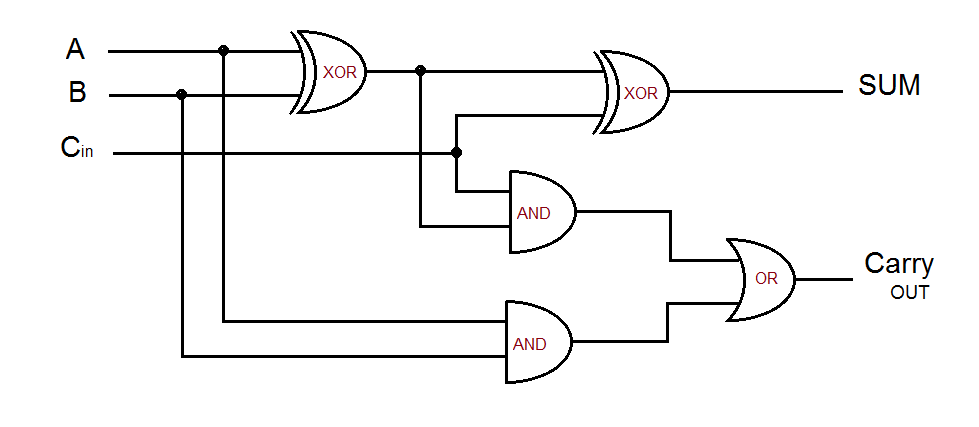
\includegraphics[width=7.5cm]{adder.png}
        \captionof{figure}{1-Bit Adder Circuit}
    \end{center}

    The 1-bit adder circuit shown above is implemented my submitted deliverable. By tracing the inputs for A, and B as the result of the multiplexer through the adder circuit, we can verify that it produces the correct outputs for the chosen operation.

    Using the example of all true inputs, the result of the multiplexer would be false, since the binvert input signal would be set to true. Using A as true, and B as false, the adder would first XOR the two inputs, resulting in true. With this result, we take the XOR of the carryin with the result of the XOR of the A and the multiplexer output of B, resulting in false, since both the carryin and result of the previous XOR are true, this makes the sum 0, with a carryout.

    Now, to compute the carryout, we take the AND of the result of the XOR of the A and the multiplexer output of B, resulting in true, and then taking the AND of A and the multiplexer output of B, resulting in false, since A is true and the result of the multiplexer is false. Further, we OR the output of the two previous ANDs, resulting in true since one is true and the other is false. This will return a true carryout, which is the correct result for this example case.

    \begin{table}[!htb]
        \centering
        \begin{tabular}{|c|c|c|c|c>{\columncolor{green!20}}c>{\columncolor{green!20}}c|}
            \hline
            \textbf{op} & \textbf{a} & \textbf{b} & \textbf{cin} & \textbf{bneg} & \textbf{cout} & \textbf{res} \\ \hline
            01 & F & F & F & F & F & 0 \\ \hline
            01 & T & F & F & F & F & 1 \\ \hline
            01 & F & T & F & F & F & 1 \\ \hline
            01 & T & T & F & F & T & 0 \\ \hline
            01 & F & F & T & F & F & 1 \\ \hline
            01 & T & F & T & F & T & 0 \\ \hline
            01 & F & T & T & F & T & 0 \\ \hline
            01 & T & T & T & F & T & 1 \\ \hline
            01 & F & F & 0 & T & F & 1 \\ \hline
            01 & T & F & F & T & T & 0 \\ \hline
            01 & F & T & F & T & F & 0 \\ \hline
            01 & T & T & F & T & F & 1 \\ \hline
            01 & F & F & T & T & T & 0 \\ \hline
            01 & T & F & T & T & T & 1 \\ \hline
            01 & F & T & T & T & F & 1 \\ \hline
            01 & T & T & T & T & T & 0 \\ \hline
        \end{tabular}
        \caption{Adder Output Table}
    \end{table}
    
    \break
    \item \textbf{Op[3] — No-Op}
    $\hfill \break$
    \\
    The no-op operation is correct since the output should always be zero according to the provided circuit diagram.

    Therefore, since all of the other outputs have already been verified to work correct in the previous explanations, all components of the no-op operation are correct as shown below.

    \begin{table}[!htb]
        \centering
        \begin{tabular}{|c|c|c|c|c>{\columncolor{green!20}}c>{\columncolor{green!20}}c|}
            \hline
            \textbf{op} & \textbf{a} & \textbf{b} & \textbf{cin} & \textbf{bneg} & \textbf{cout} & \textbf{res} \\ \hline
            01 & F & F & F & F & F & 0 \\ \hline
            01 & T & F & F & F & F & 0 \\ \hline
            01 & F & T & F & F & F & 0 \\ \hline
            01 & T & T & F & F & T & 0 \\ \hline
            01 & F & F & T & F & F & 0 \\ \hline
            01 & T & F & T & F & T & 0 \\ \hline
            01 & F & T & T & F & T & 0 \\ \hline
            01 & T & T & T & F & T & 0 \\ \hline
            01 & F & F & 0 & T & F & 0 \\ \hline
            01 & T & F & F & T & T & 0 \\ \hline
            01 & F & T & F & T & F & 0 \\ \hline
            01 & T & T & F & T & F & 0 \\ \hline
            01 & F & F & T & T & T & 0 \\ \hline
            01 & T & F & T & T & T & 0 \\ \hline
            01 & F & T & T & T & F & 0 \\ \hline
            01 & T & T & T & T & T & 0 \\ \hline
        \end{tabular}
        \caption{No-Op Output Table}
    \end{table}
    
\end{itemize}

\end{document}
